\documentclass[tikz,convert={density=150,size=600,outext=.png}]{standalone}
\usetikzlibrary{shapes, calc, arrows, fit, positioning, decorations, patterns, decorations.pathreplacing, chains, snakes}

\begin{document}
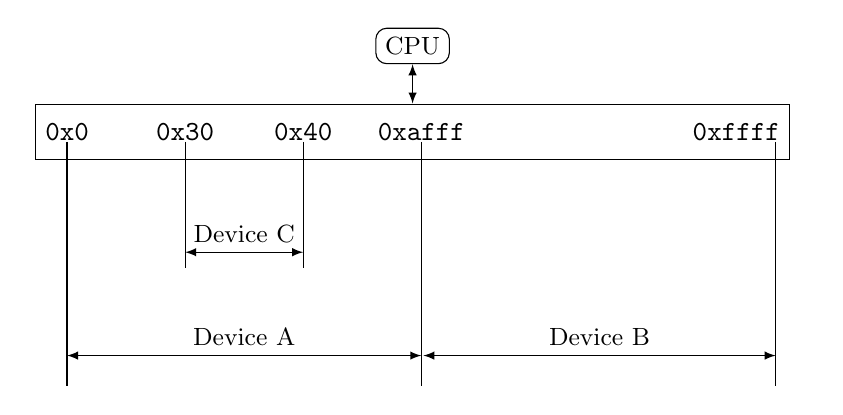
\begin{tikzpicture}[font=\small, >=latex]
    \path[font=\ttfamily, inner xsep=0pt] (0,0) -- (10,0) node[pos=0.05, above] (0x0) {0x0} node[pos=0.2, above] (0x30) {0x30} node[pos=0.35, above] {0x40} node[pos=0.5,above] (midpoint) {0xafff} node[pos=0.9, above] (0xffff) {0xffff};
    \node[draw, fit=(0x0) (0xffff)] (ruler) {};
    \node[draw, rounded corners, above=0.5cm of ruler] (cpu) {CPU};
    
    \draw[<->] (cpu) -- (ruler);
    
    \draw (2,0.1) -- (2,-1.5) coordinate[very near end, inner sep=0pt] (left-c) {};
    \draw (3.5,0.1) -- (3.5,-1.5) coordinate[very near end, inner sep=0pt] (right-c) {};
    
    \draw (0.5,0.1) -- (0.5,-3) coordinate[very near end, inner sep=0pt] (left-a) {};
    \draw (5,0.1) -- (5,-3.) coordinate[very near end, inner sep=0pt] (right-a) {} node[very near end, inner sep=0pt] (left-b) {};
    \draw (9.5,0.1) -- (9.5,-3) coordinate[very near end, inner sep=0pt] (right-b) {};
    
    \draw[<->] (left-c) -- (right-c) node[midway, above] (dev-c) {Device C};
    \draw[<->] (left-a) -- (right-a) node[midway, above] (dev-a) {Device A};
    \draw[<->] (left-b) -- (right-b) node[midway, above] (dev-b) {Device B};
\end{tikzpicture}

\end{document}
